\documentclass[10pt,a4paper]{article}
\usepackage[utf8]{inputenc}
\usepackage{amsmath}
\usepackage{amsfonts}
\usepackage{amssymb}

\usepackage{float}
\usepackage[table,xcdraw]{xcolor} %para usar tablas con color de fondo en las celdas
\usepackage{hyperref} %para poder poner enlaces
\usepackage{listings} %para insertar código
\usepackage{tikz}%para pintar las redes neuronales
\usepackage{color} %para poder definir y usar colores
\usepackage{soul} %para hacer los subrayados

\author{\textbf{Gustavo Rivas Gervilla}}
\title{\textcolor{deepblue}{\textbf{Agoritmos Genéticos para QAP}}}
\date{}

%Configurando lstlisting para mostrar código Python con algún 	 de colores (copiado de http://tex.stackexchange.com/questions/83882/how-to-highlight-python-syntax-in-latex-listings-lstinputlistings-command) ------------------------------
% Custom colors
\definecolor{deepblue}{rgb}{0,0,0.5}
\definecolor{deepred}{rgb}{0.6,0,0}
\definecolor{deepgreen}{rgb}{0,0.5,0}
\definecolor{light-gray}{gray}{0.85}
\definecolor{comment-gray}{gray}{0.65}
\definecolor{light-green}{rgb}{0.66,1,0.5}
\definecolor{light-yellow}{rgb}{1,1,0.4}

% Default fixed font does not support bold face
\DeclareFixedFont{\ttb}{T1}{txtt}{bx}{n}{8} % for bold
\DeclareFixedFont{\ttm}{T1}{txtt}{m}{n}{8}  % for normal

%Configuración de los listings
\lstset{
	language=Python,
	basicstyle=\ttm,
	otherkeywords={self},             % Add keywords here
	keywordstyle=\ttb\color{deepblue},
	emph={MyClass,__init__},          % Custom highlighting
	emphstyle=\ttb\color{deepred},    % Custom highlighting style
	stringstyle=\color{deepgreen},
	frame=tb,                         % Any extra options here
	showstringspaces=false,            % 
	commentstyle=\ttm\color{comment-gray}, % Custom comment style
}
%--------------------------------------------------------------------------------

\newcommand{\emp}[1]{\sethlcolor{light-yellow}\hl{\texttt{#1}}} %Comando para poner código inline
\newcommand{\code}[1]{\sethlcolor{light-gray}\hl{\texttt{#1}}} %Comando para poner código inline
\newcommand{\archive}[1]{\sethlcolor{light-green}\hl{\texttt{#1}}} %Comando para resaltar nombres de archivos
\renewcommand\tablename{Tabla} %Cambiar el nombre de las tablas
\renewcommand\figurename{Figura} %Cambiar el nombre de las tablas
\renewcommand{\contentsname}{Índice} %Cambiar el nombre de la ToC

\begin{document}
\maketitle
\begin{center}
\textbf{IC. Máster Universitario en Ingeniería Informática}
\newline
\newline
\newline

\includegraphics[scale=0.5]{img/decsai}
\end{center}

\newpage
\tableofcontents
\newpage

%Definición de variables para tikz
\def\layersep{2.5cm}

\section{Introducción}

En esta práctica nos enfrentamos al problema de la asignación cuadrática (QAP), empleando para su resolución algoritmos genéticos. Nos enfrentamos a diversos problemas, aunque el que realmente nos ocupa es el \code{tai256c} ya que es el que se emplea para establecer el ranking de puntuación de la parte de competición de esta práctica.\\

Este problema tiene un espacio de búsqueda de 256! elementos con lo que es evidente que una estrategia de fuerza bruta no es viable. Por lo tanto una solución basada en algoritmos genéticos es una buena aproximación para esta resolución, pese a que otros algoritmos son los que han obtenido la mejor solución al problema tai256c. Veamos cómo hemos abordado esta práctica.\\

También se considerarán dos variables meméticas del algoritmos genéticos usual, las variantes balwiniana y lamarckiana, haciendo uso del algortimos 2-opt para el proceso de optimización local de soluciones.

\section{Implementación}

Para la implementación de los algoritmos necesarios para esta práctica nuevamente hemos optado por \code{Python 3.6}, en esta ocasión sin hacer uso de la librería Theano para hacer cálculos matrices optimizados, pese a que hemos tenido algunos problemas de rendimiento que se detallarán más adelante, en un inicio no se consideró necesario y por tanto no se ha incorporado esta librería.\\

Sí que hemos hecho uso de \code{Numpy} ya que para los cálculos matrices resulta mucho más eficiente que implementar el bucle doble pertinente, de hecho ya veremso el problema que nos ha supuesto el uso de un bucle doble en nuestro código. Señalar que la versión de este módulo es \code{Numpy 1.11.3}, en el ordenador de sobremesa teníamos otra versión anterior y el programa no funcionaba correctamente, en concreto al crear con la función \code{random.permutation}, los resultados no eran correctos.

\subsection{Elementos del algoritmo genético básico}

La \textbf{representación} que hemos empleado para los cromosomos es la usual, una permutación de n elementos siendo n el número de localizaciones y unidades que componen el problema. Así, si nos ceñimos al problema original del QAP, cada elementos de la permutación sería la localización en la que situaríamos la unidades correspondiente a ese índice de la permutación.\\

El \textbf{operador de cruce} empleado ha sido el OX de uso muy extendido. Otro operador de cruce muy usado es el denominado PMX pero hemos optado por este primero por la facilidad de su implementación. Por otro lado el \textbf{operador de mutación} es simplemente el intercambio en de valores entre dos elementos de la permutación.\\

Como operador de selección empleamos torneo binario, para ello aprovechamos que ordenamos los padres de modo que el generar números aleatorios para seleccionar los padres lo hacemos generando un número aleatorio y a continuación otro menor o igual que él, que será el padre que seleccionemos para cruce como resultado del torneo. Hablaremos de esto en la siguiente subsección.

\subsection{Algunas consideraciones}

\begin{enumerate}
\item Un problema que hemos encontrado es que durante la ejecución del algoritmo, en concreto el lamarckiano, que es el que hemos empleado para tratar de obtener una buena solución en el tai256c, se producían fluctuaciones en el fitness de las soluciones. Esto creo que se debe a haber empleado floats para almacenar las soluciones así como las matrices del problema con el objetivo de hacer un código más genérico. No obstante se cambió el código de modo que ahora se emplean enteros de 64 bits y no parece que se dé este problema.
\item Debido al mecanismo empleado para leer las matrices de los ficheros de datos es necesario que haya una línea en blanco entre cada uno de los elementos del problema; las dos matrices y la dimensión del problema. Así por ejemplo se han realizado estas modificaciones en los archivos de tai que se han empleado para la realización de esta práctica.
\item Otro problema que hemos tenido ha sido la elección del lenguaje de programación, como ya dijo el profesor Python puede resultar lento, peso a que este problema podemos solventarlo haciendo uso de librerías externas como Numpy, no obstante el bucle doble, que se ha escrito para programar el algoritmo 2opt hace que una ejecución de este algoritmo sobre una instancia del tai256 duré más de un minuto, con lo cuál en una población de 100 individuos que es la que se ha considerado en las experimentaciones, esto se traduciría en un mínimo de 100 minutos por generación algo que no se podía abordar si queríamos obtener resultados tras varias generaciones del algoritmo.\\

En ocasiones las variantes lamarckiana y balwiniana se basan en aplicar el proceso de optimización sólo a algunos elementos de la población, y esta ha sido la opción que hemos elegido. En concreto, y tras alguna experimentación que comentaremos en la sección siguiente, aplicamos los procesos de optimización a los 20 mejores individuos de la población. Además se ha hecho uso del módulo \code{multiprocessing} que nos permite realizar cálculos en paralelo en cada uno de los núcleos (lógicos) de nuestro ordenador. Así en nuestro caso podemos realizar hasta 8 proceso de optimización simultáneamente, reduciendo así el tiempo tomado por cada generación del algoritmo.

\item Teniendo en cuenta que habrá ciertos operadores de cruce o probabilidades de cruce y mutación que exploren mejor el espacio de búsqueda, también es cierto que influye el azar en este tipo de algoritmos. Así que para poder ejecutar un gran número de ejecuciones del algoritmo sobre el mismo conjunto de datos lo que hemos hecho ha sido almacenar, tanto las mejores soluciones encontradas durante el proceso, como las generaciones producidas, cada 10. Así en un momento dado se puede parar el algoritmo y retomarlo en el punto en el que se dejó.\\

Es claro que para poder repetir los experimentos no basta con fijar una semilla aleatoria al inicio, habrá que realizar las iteraciones en las mismas ejecuciones en el que se realizaron, es decir, se repetirían las ejecuciones del algoritmo en los mismos bloques en los que se realizaron originalmente, de modo que la semilla aleatoria siempre dé los mismo resultados. Los archivos con las generaciones podemos encontrarlo en el directorio \archive{lamarck20BestGenerations}. Y el código relativo a la carga de una generación almacenada y el almacenamiento de las nuevas producidas está comentado en el archivo \archive{GAlamarck.py}.

\item En cuanto a la generación de número aleatorios para el cruce y la mutación lo que hacemos es algo que aprendimos en Metaheurísticas. Dado que la generación de números aleatorios puede ser muy costosa, en lugar de generar un número aleatorio para por ejemplo cada padre y cromosoma para ver si lo mutamos o no. Lo que hacemos es calcular cuántos cruces y mutaciones se realizarán en media en cada generación y hacemos siempre este número fijo. De modo que sólo hemos de generar esta cantidad fija de números aleatorios en cada generación y no la cantidad que se generaría si lo hiciésemos de la forma usual. Por esto en el código tenemos las variables \code{nCrosses} y \code{nMutations}.
\end{enumerate}

\section{Experimentación}

Debido a los problemas debidos al tiempo de cómputo necesario tomado por los algoritmos se ha decidido realizar una comparativa de los distintos algoritmos sobre un problema más pequeño el \code{tai60a}. Comenzamos en primer lugar a realizar experimentos sobre un grid de parámetros para el algoritmo genético básico, experimentos que se repetirán para los dos variantes de este algoritmo.

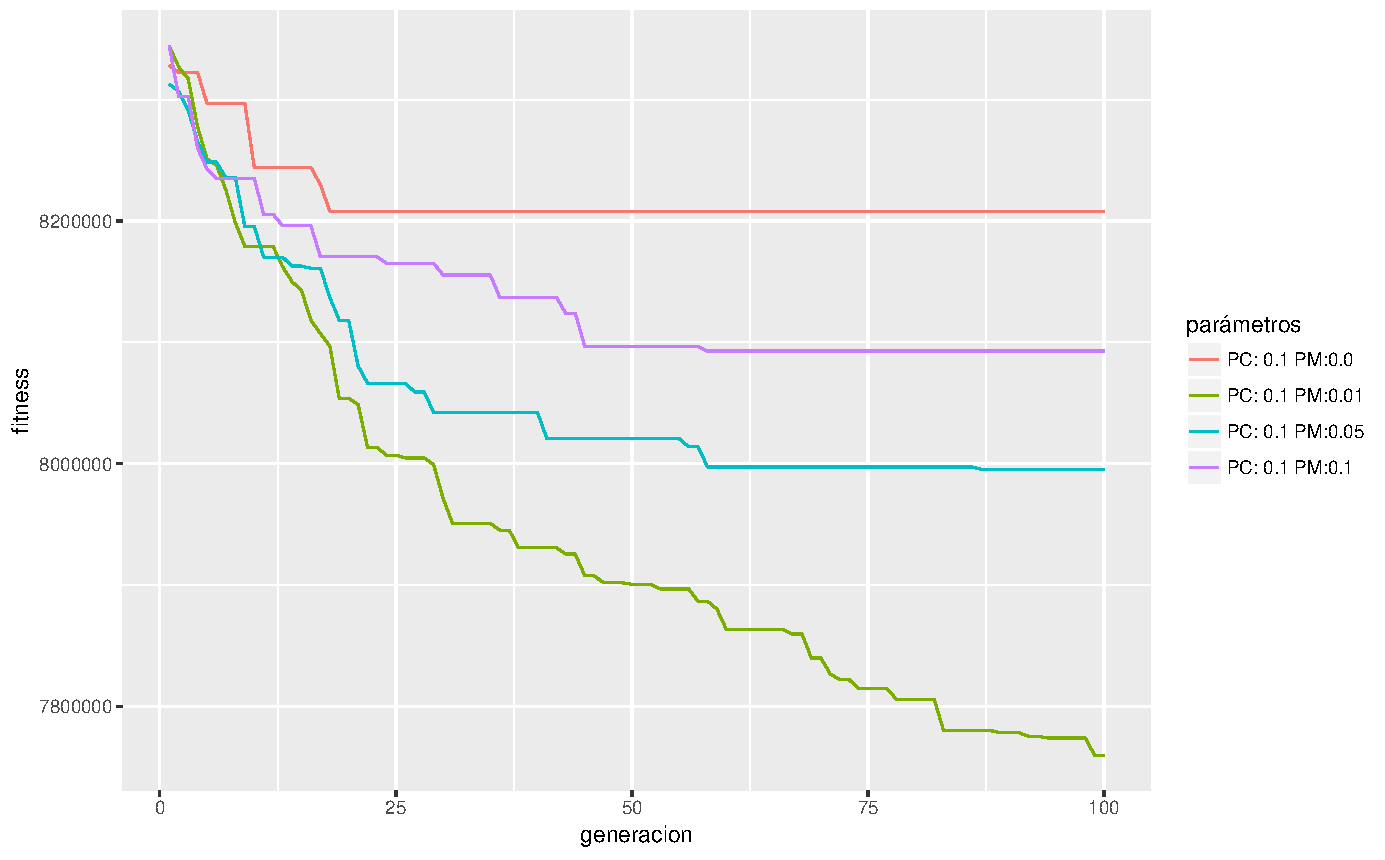
\includegraphics[width = \textwidth]{img/graphics/GAgenericPC01.pdf}
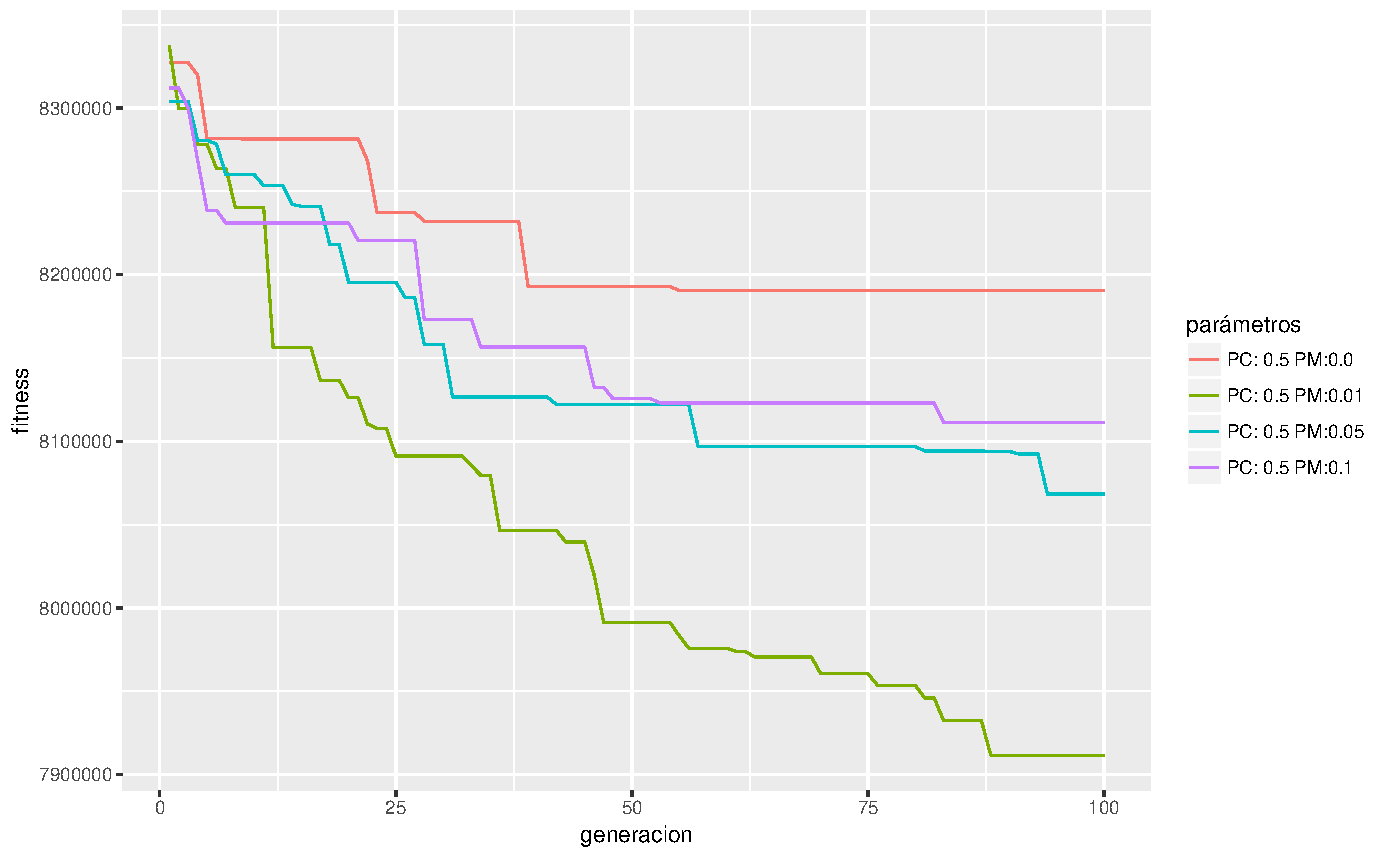
\includegraphics[width = \textwidth]{img/graphics/GAgenericPC05.pdf}
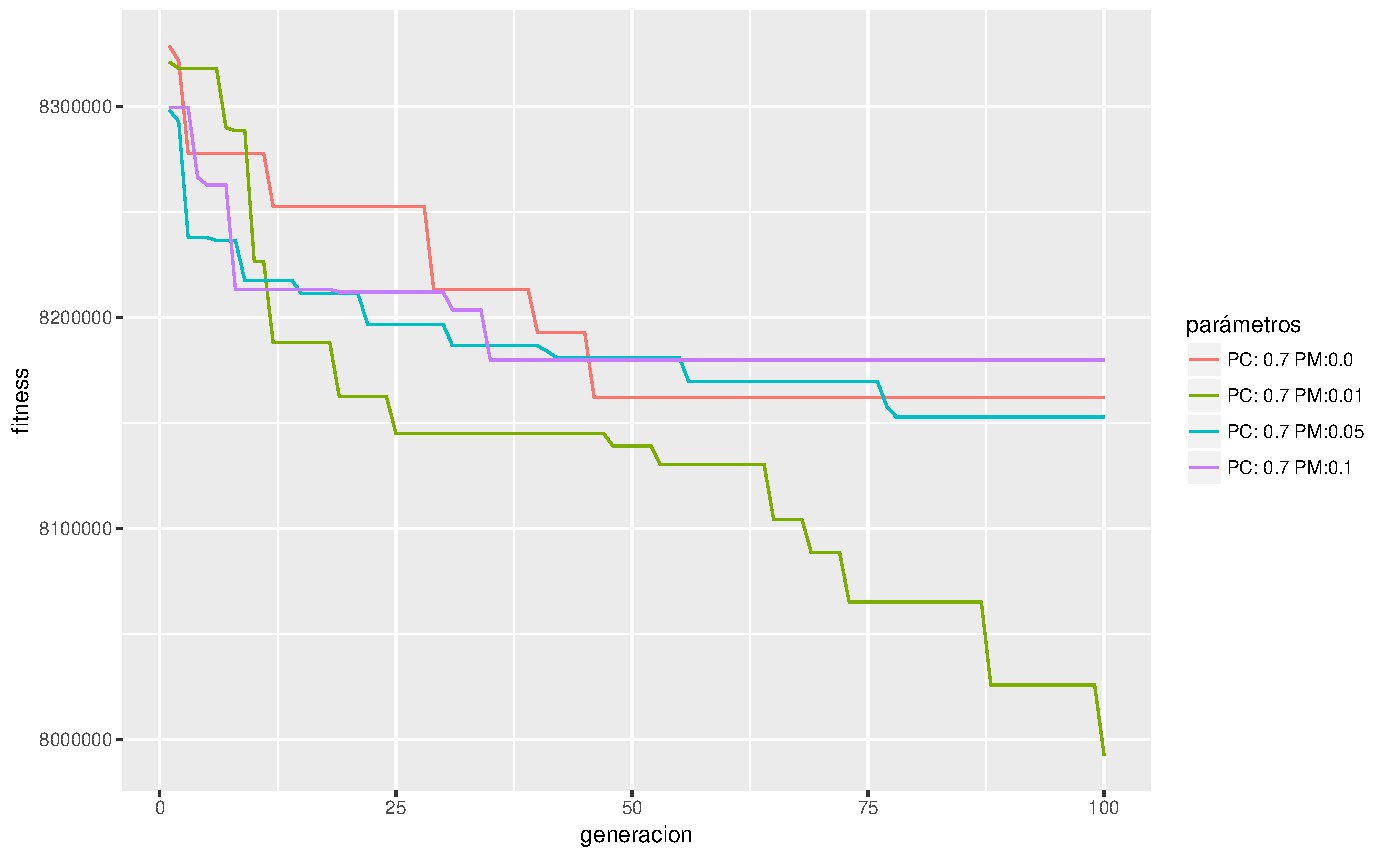
\includegraphics[width = \textwidth]{img/graphics/GAgenericPC07.pdf}

En estas gráficas podemos observar algo y es que en un principio, para una misma probabilidad de cruce (que sería en media el número de cruces que haríamos por generación) es malo tanto una probabilidad de mutación baja, hemos probado a no poner ninguna mutación y con lo cual se observa que el algoritmo se queda estancado. Como una probabilidad de mutación demasiado alta, en este caso las probabilidades 0.05 y 0.1 han resultado perjudiciales para la exploración del algoritmo. Este hecho puede deberse a que lo que hacemos con un número de mutaciones muy elevado es perder las propiedades o genes buenos de los cromosomas de nuestra población, no siendo capaces de encontrar una mejor solución a partir de ellos. Así la mejor probabilidad para este problema, de las 4 que hemos probado, es 0.1.

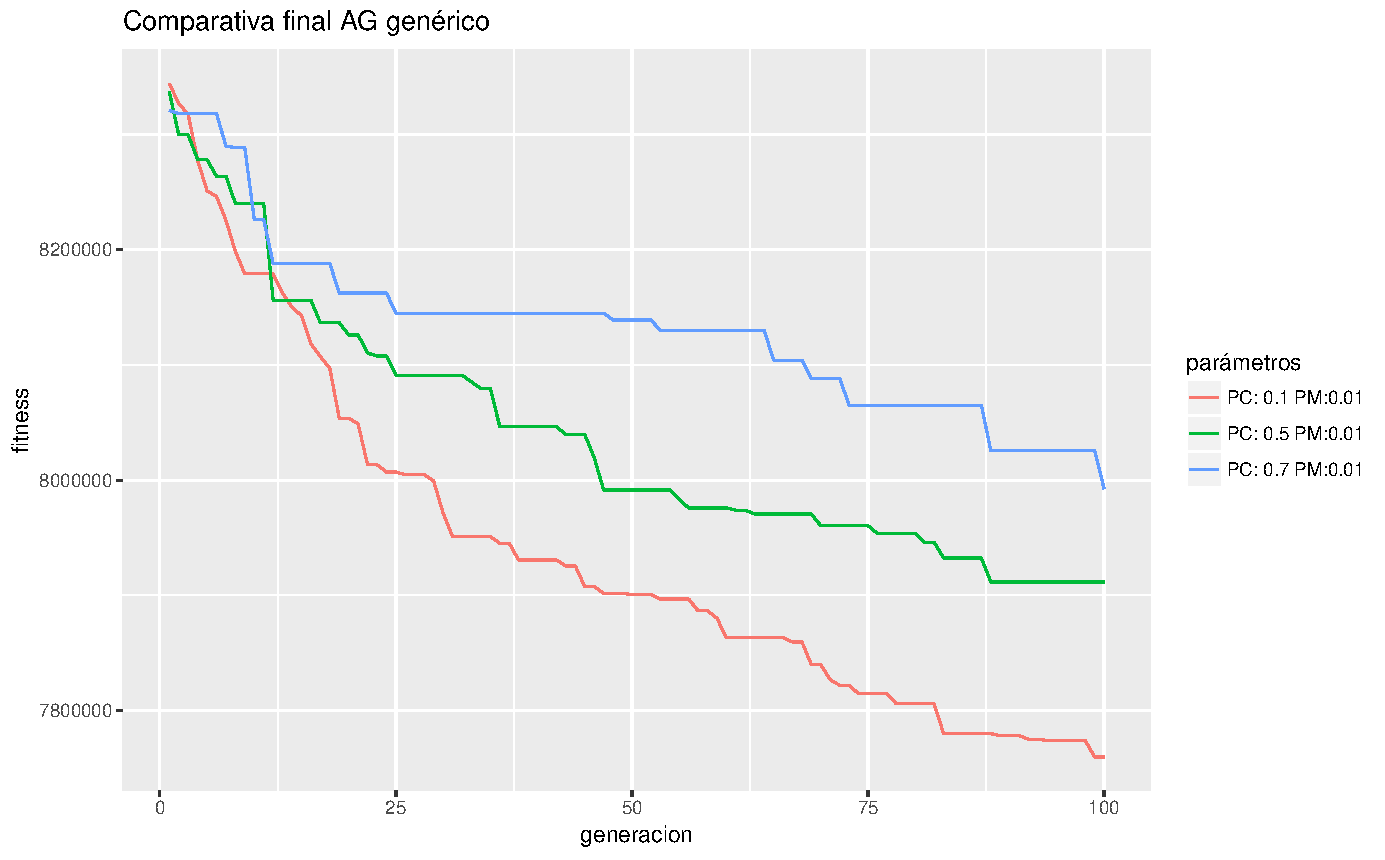
\includegraphics[width = \textwidth]{img/graphics/GAgenericFinal.pdf}

Y aquí vemos cómo, una vez que fijamos la probabilidad de mutación a la mejor de las 4 probadas, cuánto menor es la probabilidad de cruce mejor es el resultado que podemos obtener. El cruce no deja de ser otra fuente de diversidad en nuestro algoritmo, con lo que este hecho puede darse por una razón similar a la que hemos expuesto anteriormente para la probabilidad de mutación.\\

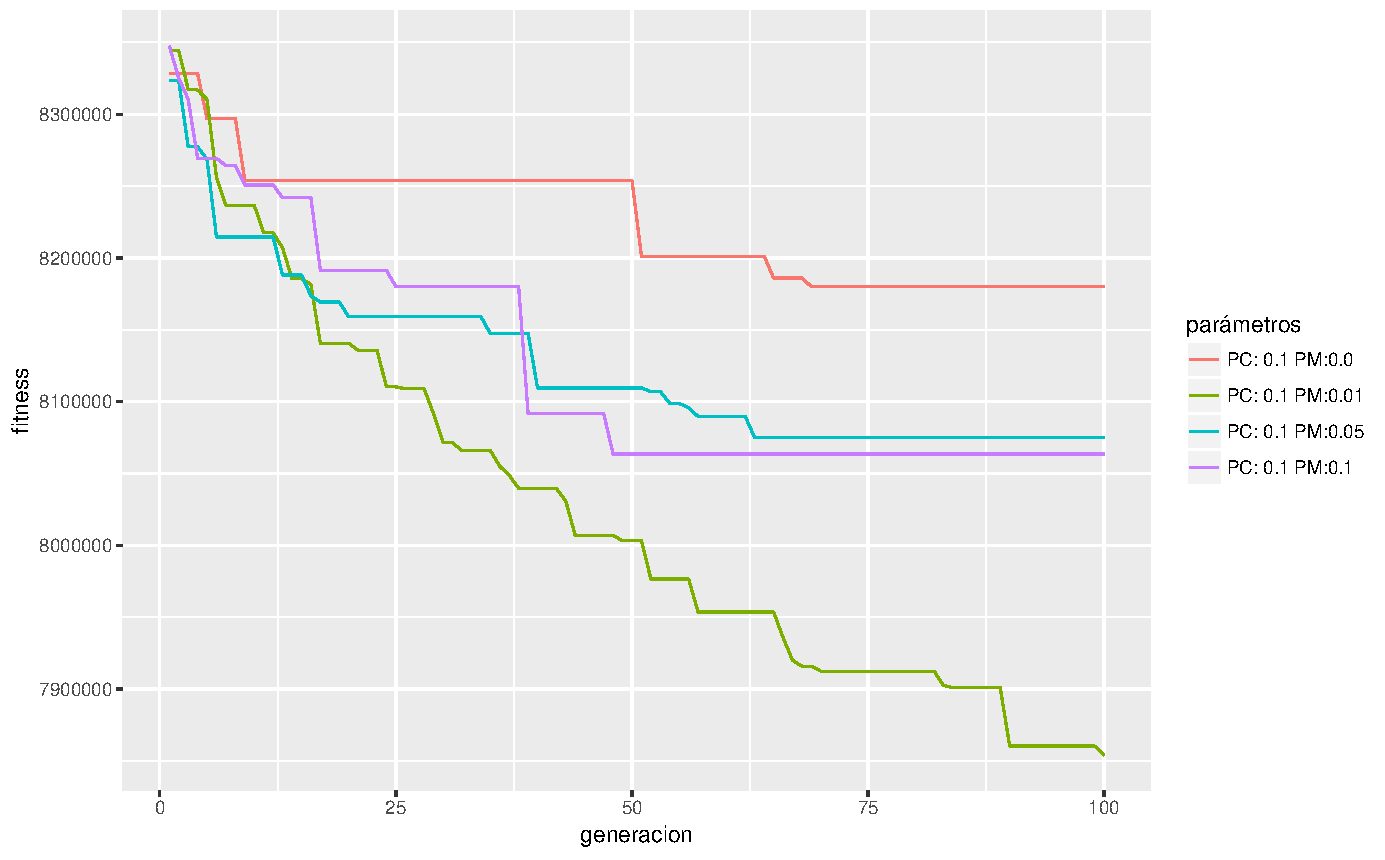
\includegraphics[width = \textwidth]{img/graphics/GAbaldwinPC01.pdf}
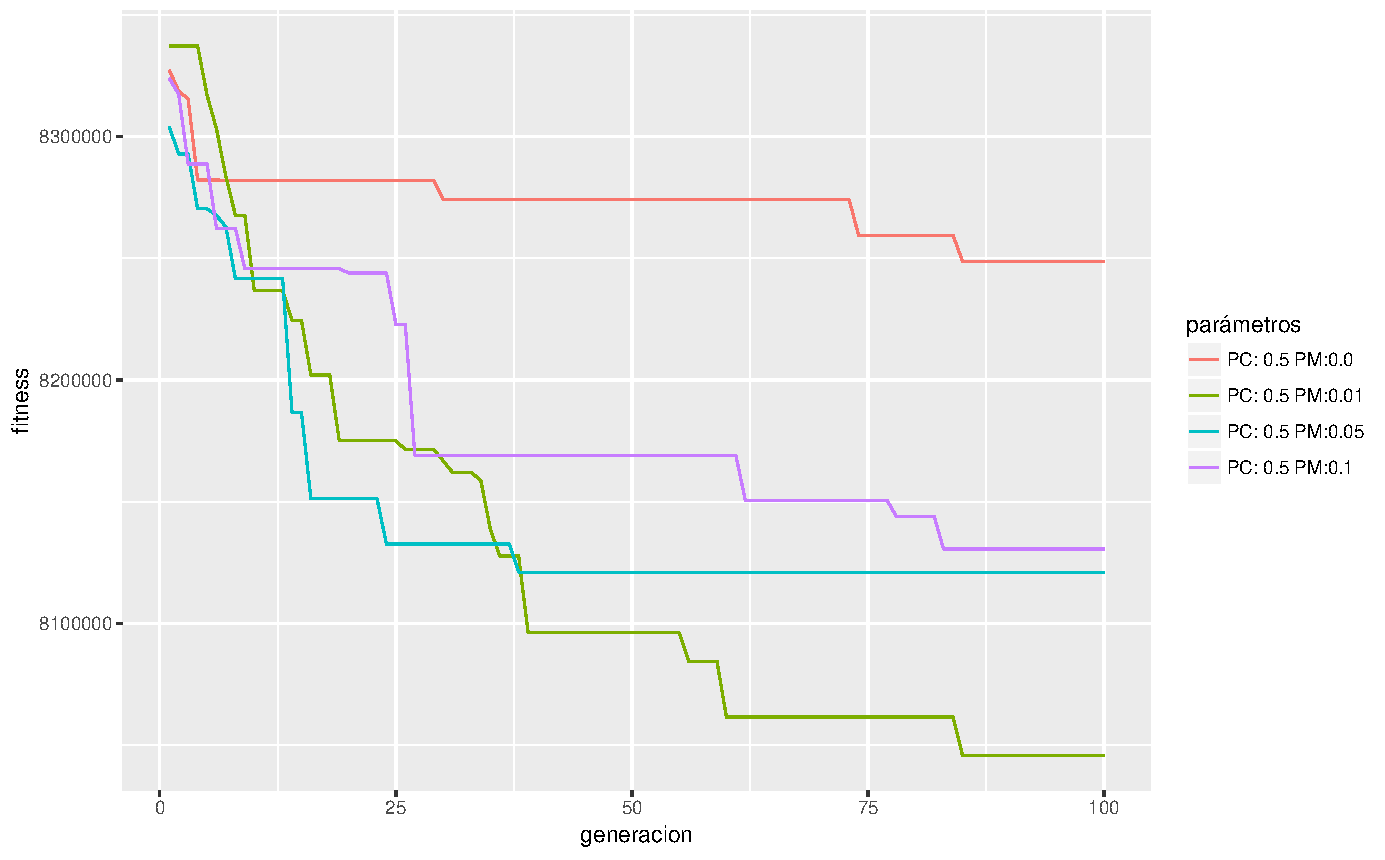
\includegraphics[width = \textwidth]{img/graphics/GAbaldwinPC05.pdf}
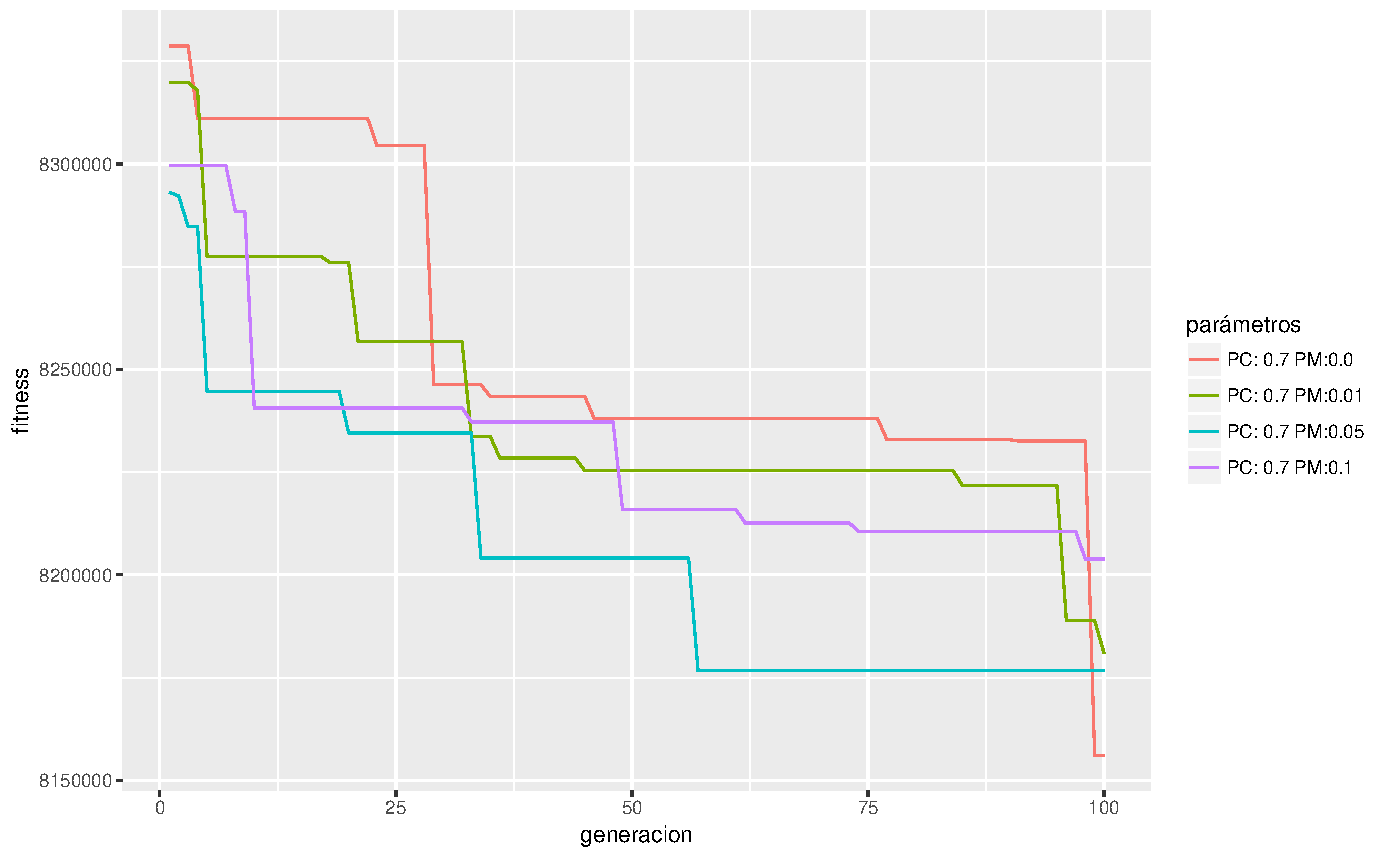
\includegraphics[width = \textwidth]{img/graphics/GAbaldwinPC07.pdf}
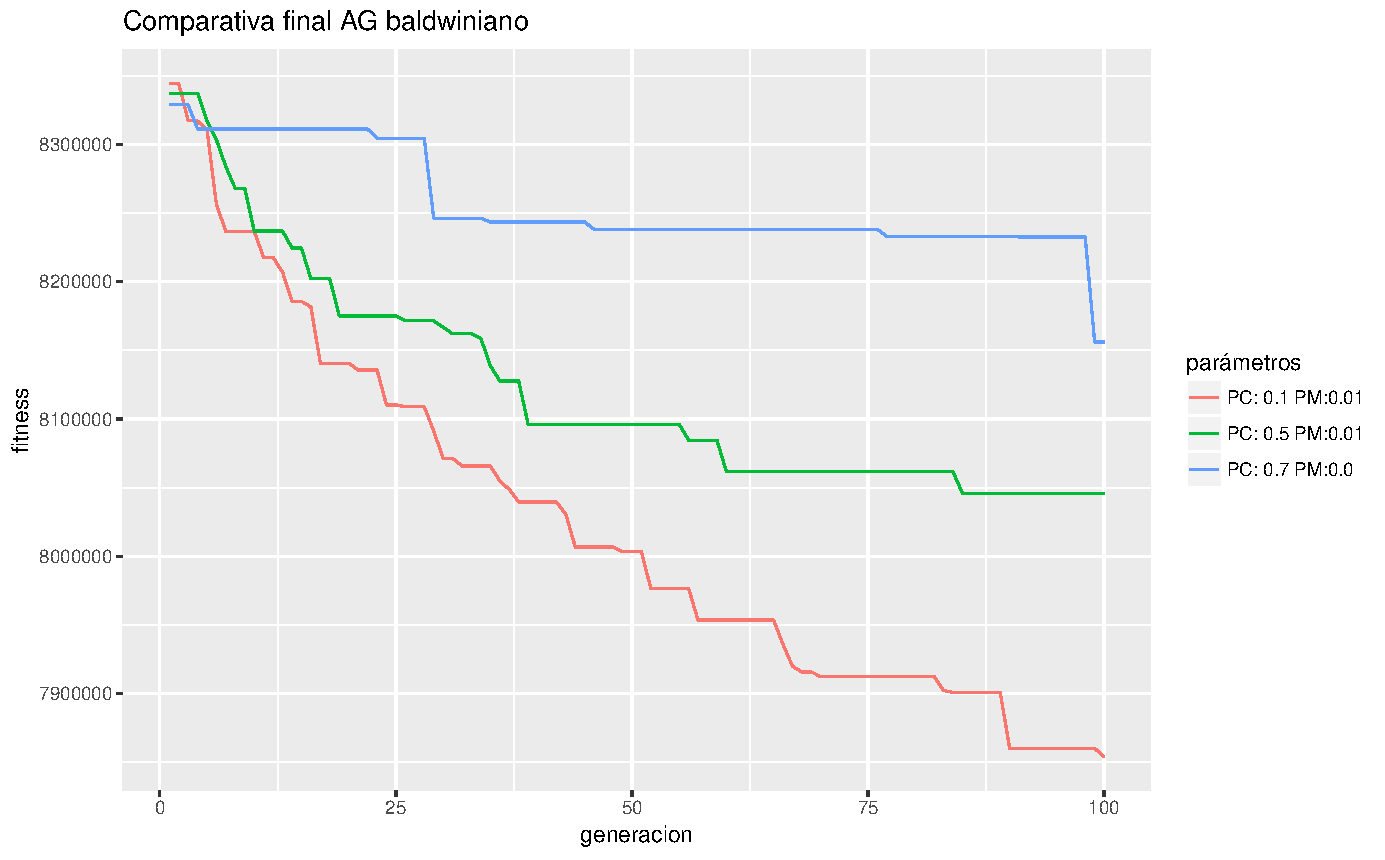
\includegraphics[width = \textwidth]{img/graphics/GAbaldwinFinal.pdf}

Aquí sucede algo extraño y es que cuando la probabilidad de cruce es alta, 0.7, entonces es cuando mejor funciona el algoritmo si no hacemos ningún tipo de mutación. Esto puede implicar que los mejores individuos de la población llegan, a través del proceso de optimización, a buenas soluciones y que participando en el corte con más frecuencia dan lugar a muy buenas soluciones. Además nos bastacon la variabilidad de que nos da el cruce, de hecho el mutar las soluciones hace que pierdan sus buenas facultades.\\

No obstante hemos de señalar que estamos aplicando la variante baldwiniana de una forma extraña al sólo calcular el fitness ``prometedor'' para ciertos elementos de la población y no para todos. Como lo aplicamos sobre los mejores elementos en principio no debería tener un comportamiento muy distinto al algoritmo genérico más que reordenar estos mejores individuos en función de su potencial. Desgraciadamente debido a la mala elección en el lenguaje de programación, como ya hemos dicho, no hemos podido aplicar el proceso de optimización a todos los individuos de la población.

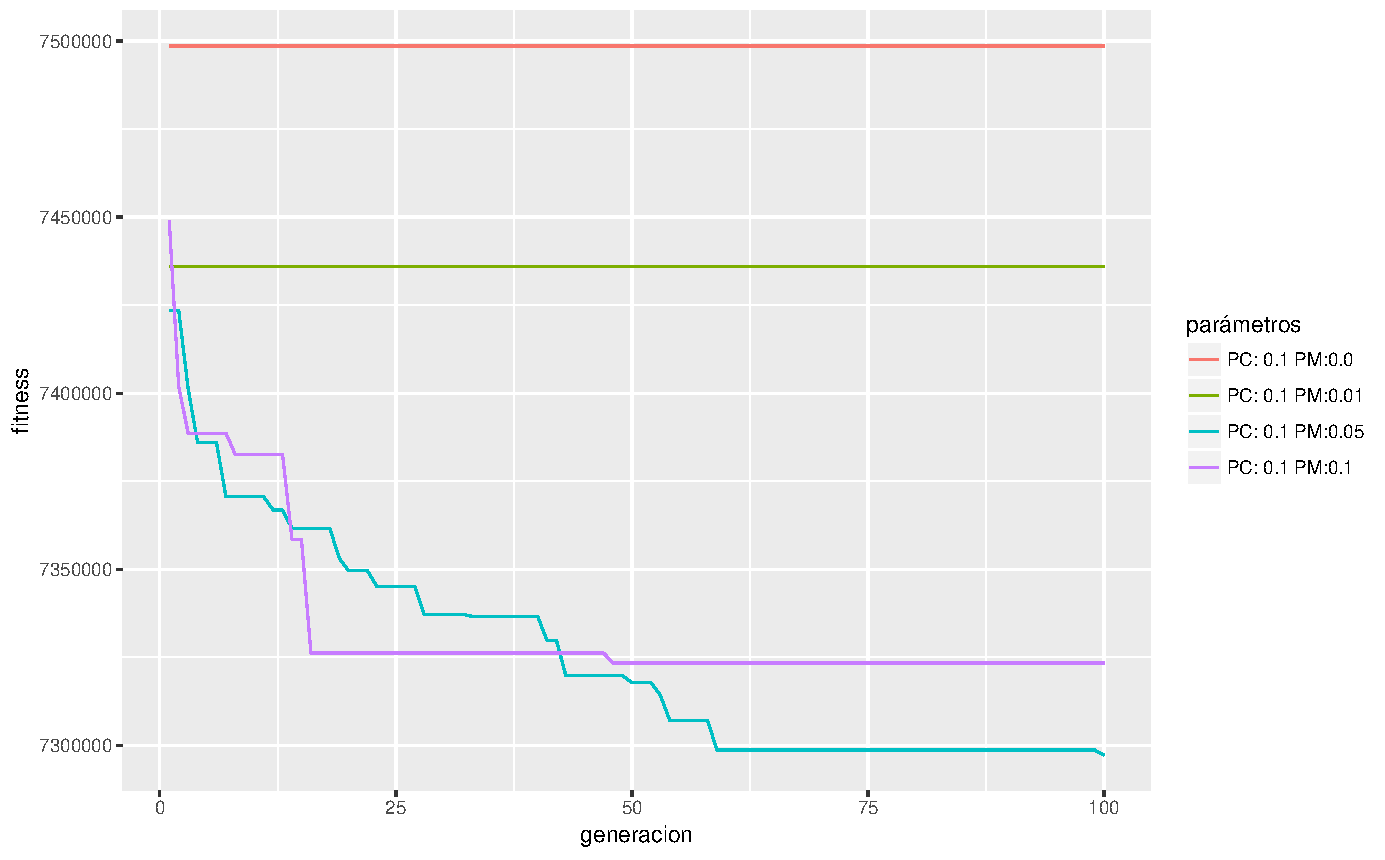
\includegraphics[width = \textwidth]{img/graphics/GAlamarckPC01.pdf}
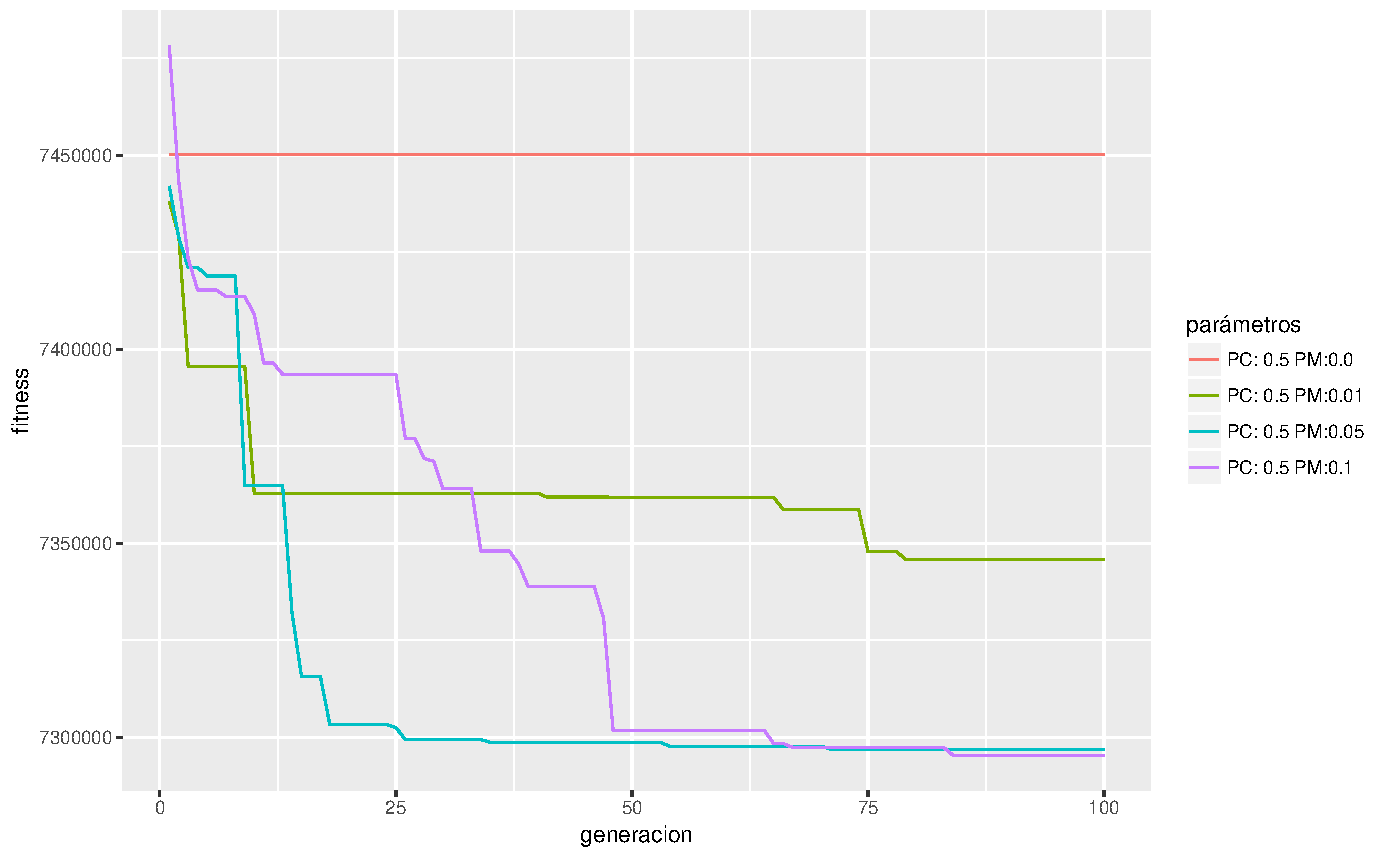
\includegraphics[width = \textwidth]{img/graphics/GAlamarckPC05.pdf}
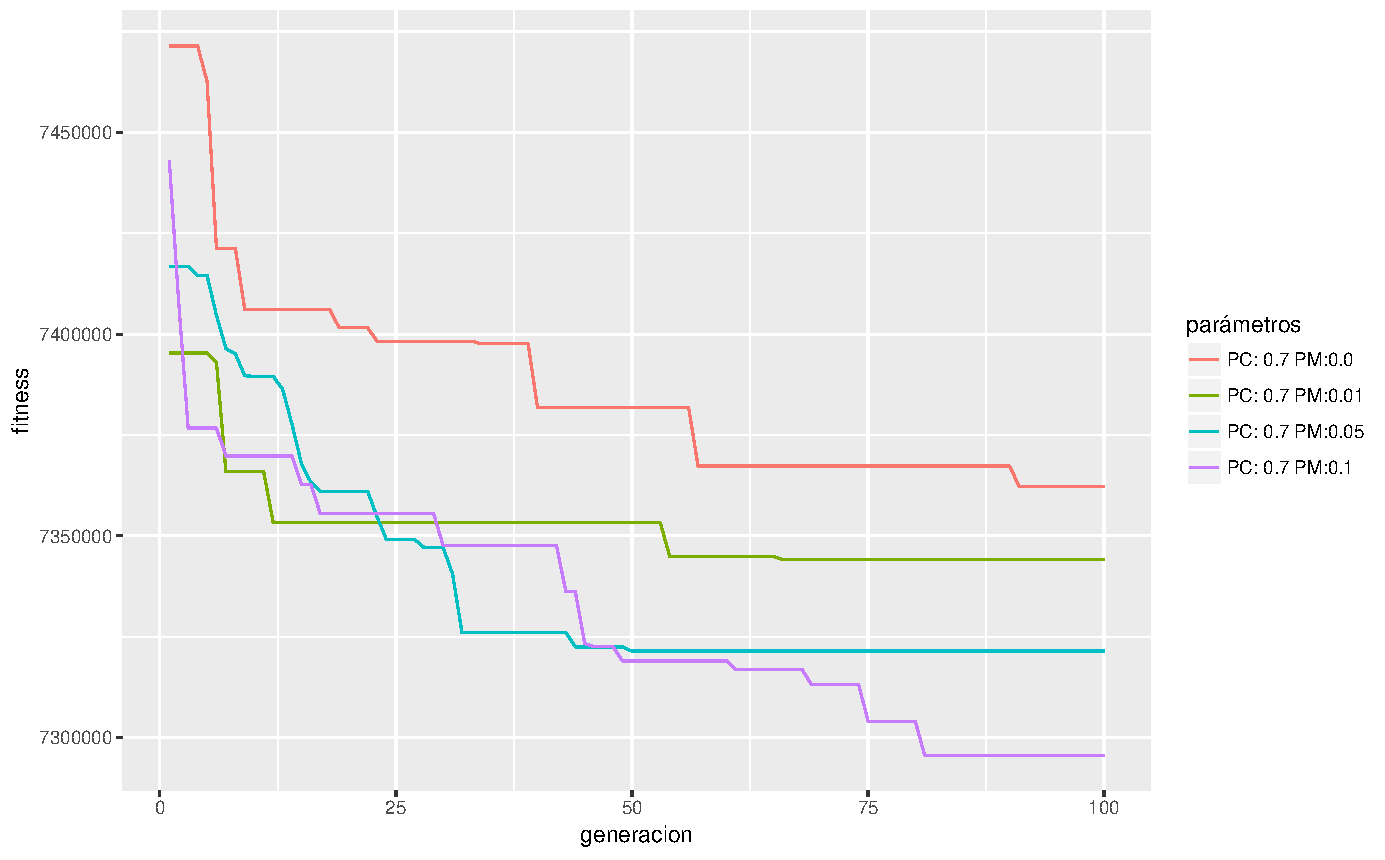
\includegraphics[width = \textwidth]{img/graphics/GAlamarckPC07.pdf}
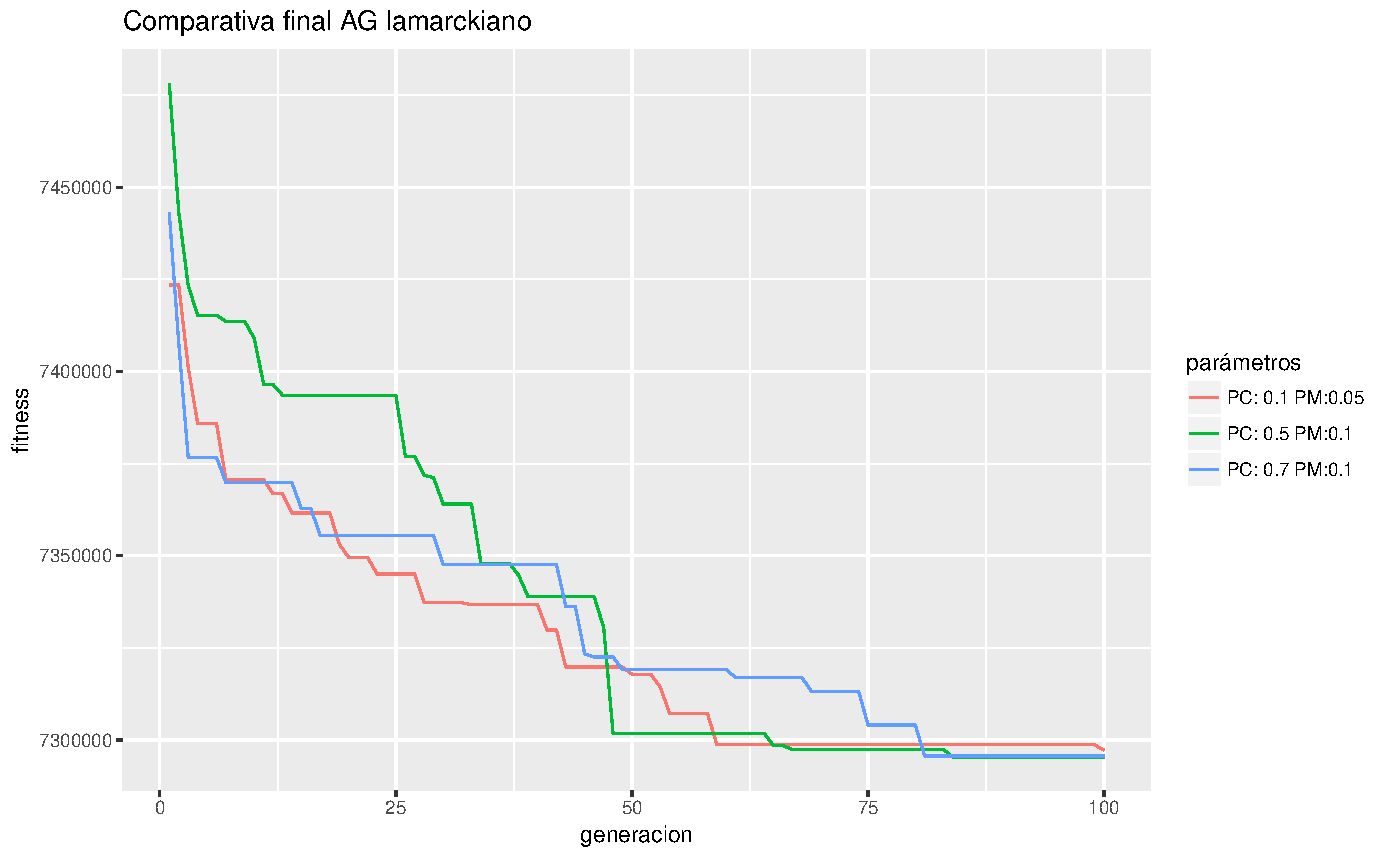
\includegraphics[width = \textwidth]{img/graphics/GAlamarckFinal.pdf}

Aquí lo que apreciamos es que, dado que el espacio de búsqueda es más pequeño que en el \code{tai256c}, el aplicar el lamarckiano puede abocarnos a un mínimo local muy rápidamente, de hecho en todos los casos, para una probabilidad de corte, las probabilidades de mutación más altas son las que dan lugar a mejores resultados.

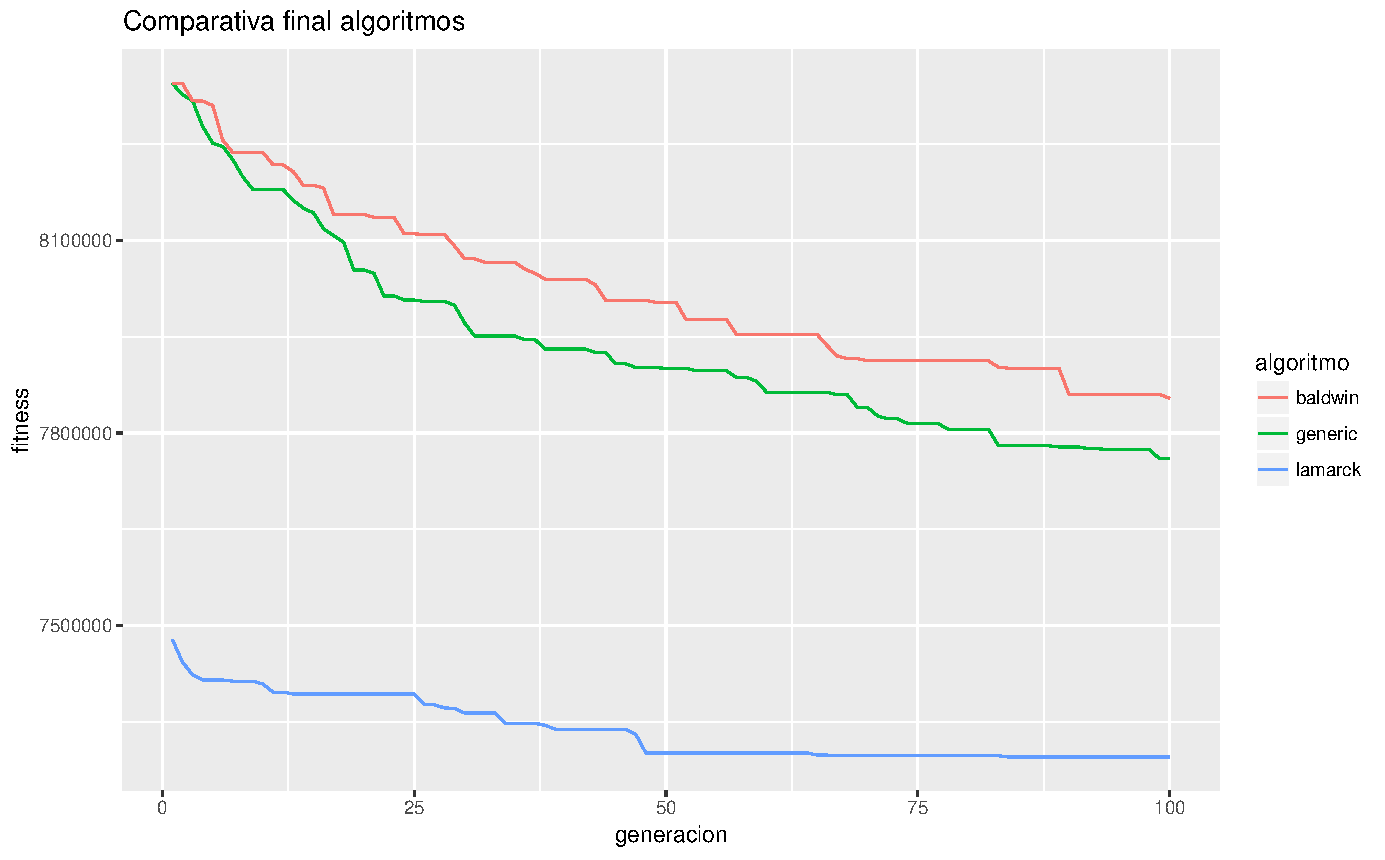
\includegraphics[width = \textwidth]{img/graphics/final.pdf}

Finalmente aquí vemos una comparativa de los tres algoritmos. Vemos como es el lamarckiano el que obtiene mejores resultados con diferencia, esto tiene sentido ya que realiza un proceso de explotación más intenso y las soluciones que encuentra en durante este proceso las incorpora en la población. En cambio como ya adelantemos anteriormente el comportamiento del algoritmo genérico y el baldwiniano es muy similar, de hecho encontramos que es el genérico el que mejor se comporta. Esto puede señalar que el fitness potencial que le asociamos a los individuos de la población no es tan buen indicativo como podríamos pensar, o que no es suficiente con calcularlo para sólo los 20 individuos de la población.

\begin{center}
\begin{table}[H]
\centering
\caption{Tiempos de los experimentos anteriores (segundos)}
\label{my-label}
\begin{tabular}{|l|l|l|l|}
\hline
\rowcolor[HTML]{FFFC9E} 
\textbf{Parámetros}                 & \multicolumn{1}{c|}{\cellcolor[HTML]{FFFC9E}\textbf{Genérico}} & \multicolumn{1}{c|}{\cellcolor[HTML]{FFFC9E}\textbf{Baldwiniano}} & \multicolumn{1}{c|}{\cellcolor[HTML]{FFFC9E}\textbf{Lamarckiano}} \\ \hline
PC 0.1 PM 0                         & \multicolumn{1}{c|}{0.1965632438659668}                        & \multicolumn{1}{c|}{229.46095776557922}                           & \multicolumn{1}{c|}{40.006726026535034}                           \\ \hline
PC 0.1 PM 0.01                      & \multicolumn{1}{c|}{1.176302433013916}                         & \multicolumn{1}{c|}{237.49341559410095}                           & \multicolumn{1}{c|}{41.53278636932373}                            \\ \hline
PC 0.1 PM 0.05                      & \multicolumn{1}{c|}{4.538119792938232}                         & \multicolumn{1}{c|}{239.02621841430664}                           & \multicolumn{1}{c|}{118.29913687705994}                           \\ \hline
\multicolumn{1}{|c|}{PC 0.1 PM 0.1} & \multicolumn{1}{c|}{8.739510536193848}                         & \multicolumn{1}{c|}{238.1887505054474}                            & \multicolumn{1}{c|}{161.66303634643555}                           \\ \hline
PC 0.5 PM 0                         & 0.7903800010681152                                             & 288.2191894054413                                                 & 40.6226110458374                                                  \\ \hline
PC 0.5 PM 0.01                      & 1.835338830947876                                              & 232.97396326065063                                                & 63.90303945541382                                                 \\ \hline
PC 0.5 PM 0.05                      & 5.205590009689331                                              & 231.69750213623047                                                & 132.511292219162                                                  \\ \hline
PC 0.5 PM 0.1                       & 9.499826192855835                                              & 233.9859938621521                                                 & 175.75801801681519                                                \\ \hline
PC 0.7 PM 0                         & 1.2097265720367432                                             & 303.1206007003784                                                 & 81.32161521911621                                                 \\ \hline
PC 0.7 PM 0.01                      & 2.1152844429016113                                             & 241.62352299690247                                                & 108.90502667427063                                                \\ \hline
PC 0.7 PM 0.05                      & 5.394533395767212                                              & 241.96477484703064                                                & 163.41942262649536                                                \\ \hline
PC 0.7 PM 0.1                       & 9.53583288192749                                               & 239.10191750526428                                                & 190.24293994903564                                                \\ \hline
\end{tabular}
\end{table}
\end{center}

Lo primero que apreciamos en la tabla anterior es algo evidente, cuantos más cruces y mutaciones se realicen mayor será el tiempo de ejecución del algoritmo. Como podemos ver el algoritmo balwiniano tarda más que el lamarckiano, teóricamente deberían tardar lo mismo ya en ambos casos aplicamos el proceso de optimización a los 20 mejores elementos de la población y lo que cambia en principio es simplemente la información que tomamos de ese proceso. No obstante según se ha implementado el algoritmo baldwiniano conlleva bastante más cálculos que el lamarckiano y por esto tenemos esta diferencia de tiempos.\\

Lo que hacemos es aplicar el algoritmo de optimización a los 20 mejores elementos de la población y en lugar de preservar los cálculos realizados, debido a una mala implementación, recalculo los fitness originales de los padres que han sido optimizados para las fases de elitismo.\\

Hay que señalar que para este experimento se han empleado dos implementaciones del opt distintas a la empleada para el problema de competición, se ha observado que si en lugar de aplicar la función que usa la factorización de la función de fitness calculamos el score de los individuos de la forma original se tarda menos en ambos casos. No obstante hemos probado a hacer esto sobre un individuo del \code{tai256c} y hemos notado que se tarda prácticamente lo mismo, con lo cual hemos optado por continuar ejecutando el algoritmo con el código para el 2opt que teníamos originariamente para ese problema (el algoritmo se está ejecutando en el sobremesa sobre el problema de la competición mientras realizamos estos experimentos menores en el portátil). También puede haber variaciones en los tiempos de estos experimentos debido a que hemos empleado el portátil mientras se ejecutaban.\\

Además de hacer estos experimentos más pequeños para poder estudiar el comportamiento de los algoritmos también hemos realizado algunos experimentos orientados a la competición, es decir, sobre el problema \code{tai256c}. En concreto nos centramos en probar la variante lamarckiana.\\

En primer lugar probamos a aplicarlo sólamente una vez por generación y luego 10. Luego pasamos a realizar experimentos aplicando el 2opt a sólo los 10 peores individuos de la población obteniendo un resultado de 49900144 en dos generaciones, con una probabilidad de mutación de 0.1 y una de cruce de 0.3. Dado que la ejecución del algoritmo era muy lenta no realizamos una experimentación tan extensa. Una vez que descrubrimos el uso del módulo \code{multiprocessing} entonces se realizaron los siguientes experimentos:

\begin{center}
\begin{table}[H]
\centering
\caption{Primeros experimentos con Lamarck}
\label{my-label}
\begin{tabular}{|l|c|c|c|c|c|}
\hline
\rowcolor[HTML]{FFFC9E} 
\textbf{Fitness}               & \textbf{2-opt se aplica a}  & \textbf{\begin{tabular}[c]{@{}c@{}}Prob.\\ cruce\end{tabular}} & \textbf{\begin{tabular}[c]{@{}c@{}}Prob.\\ mutación\end{tabular}} & \textbf{\begin{tabular}[c]{@{}c@{}}Generaciones\\ completadas\end{tabular}} & \textbf{\begin{tabular}[c]{@{}c@{}}Estancado \\ desde la\\ generación\end{tabular}} \\ \hline
44878392                       & A 8 individuos al azar      & 0.3                                                            & 0.1                                                               & 12                                                                          & 2                                                                                   \\ \hline
44862524                       & A 8 individuos al azar      & 0.5                                                            & 0.2                                                               & 50                                                                          & 21                                                                                  \\ \hline
44890208                       & A los 8 peores individuos   & 0.5                                                            & 0.2                                                               & 21                                                                          & 0                                                                                   \\ \hline
\multicolumn{1}{|c|}{44854840} & A los 8 peores individuos   & 0.3                                                            & 0.1                                                               & 33                                                                          & 9                                                                                   \\ \hline
\multicolumn{1}{|c|}{44845300} & A los 8 mejores individuos  & 0.3                                                            & 0.1                                                               & 52                                                                          & 33                                                                                  \\ \hline
\multicolumn{1}{|c|}{44821204} & A los 20 mejores individuos & 0.3                                                            & 0.1                                                               & 36                                                                          & 34                                                                                  \\ \hline
\end{tabular}
\end{table}
\end{center}

A la luz de estos experimentos decidimos pasar a hacer un uso más intensivo de la variante lamarckaina aplicando el proceso de optimización sólo a los 20 mejores individuos de la población, ya hemos dicho que por el tiempo de cómputo no podíamos permitirnos el aplicar este algoritmo sobre todos los elementos de la misma. Para poder realizar diversas iteraciones del algoritmo lo que hicimos es ir almacenando las generaciones que se iban generando cada 10 de modo que pudiésemos retomar el algoritmo allí donde lo dejamos la última vez que paramos el algoritmo, también almacenamos las mejores soluciones que vamos encontrando.\\

En total se han realizado unas 407 iteraciones del algoritmo que son las que tenemos almacenadas en la carpeta \archive{lamarck20BestGenerations}. Es fácil deducir los bloques en los que se realizaron las distintas iteraciones ya que para poder tener correctamente las generaciones que se habían realizado iniciábamos la cuenta con el número de iteración siguiente a la última realizada, con lo que la última cifra del número de la generación nos da el bloque en el que se realizó. Así las iteraciones se realizaron en los siguiente bloques:

\begin{itemize}
\item 0-60
\item 61-101
\item 102-122
\item 123-223
\item 224-264 (aquí se encontró la mejor solución)
\item 265-315
\item 316-346
\item 347-407
\end{itemize}

Comenzamos con una probabilidad de cruce de 0.3 y una de mutación de 0.1, con esto llegamos a una solución con un score de \textbf{44811968}, y seguimos algunas generaciones más con el algoritmo en estas condiciones. No obstante debido a que el algoritmo parecía estar encantado decidimos entorno a la iteración 123 bajar la probabilidad de mutación a 0.02 y subir la de cruce a 0.5, tras algunas generaciones más, en la 228 encontramos la mejor solución, con un fitness de \textbf{44804670}. Se pueden consultar otras soluciones encontradas en la carpeta \archive{resultsLamarck20Best}, en el nombre del archivo tenemos las probabilidades empleadas (PC y PM), el tamaño de la población, que siempre es 100 (PS), la iteración en la que se encontró, el tiempo de ejecución (aunque no es registra el tiempo total invertido durante todos los bloques) y el fitness de la solución (score).\\

Nuevamente el algoritmo se quedó estancando y en la iteración 315 aumentamos las probabilidades de cruce y mutación (0.7 y 0.05 respectivamente) para intentar salir de este óptimo local sin ningún resultado. Y en la iteración 346 volvimos a cambiar las probabilidades a unas más bajas (0.3 y 0.01) e introdujimos un mecanismo por el que cada 10 iteraciones sin encontrar una mejor solución, se cambian los 30 peores individuos de la población (el 30\%) por unos nuevos individuos aleatorios para tratar de dar una mayor diversidad a la búsqueda, pero tampoco hemos podido obtener una mejor solución. El mecanismo de almacenamiento de generaciones y de reinicialización de la población se encuentran comentados en el código de \archive{GAlamarck.py}.


\end{document}